\documentclass{article}
\usepackage[utf8]{inputenc}
\usepackage{graphicx}
\usepackage[spanish]{babel}
\usepackage{amssymb,amsmath,geometry}
\usepackage{etoolbox} %titulo
\makeatletter %titulo
\patchcmd{\@maketitle}{\vskip 2em}{\vspace*{-3cm}}{}{} %titulo
\makeatother %titulo
\usepackage{vmargin}
\setpapersize{A4}
\setmargins{2.5cm}       % margen izquierdo
{1.5cm}                        % margen superior
{16.5cm}                      % anchura del texto
{23.42cm}                    % altura del texto
{10pt}                           % altura de los encabezados
{1cm}                           % espacio entre el texto y los encabezados
{0pt}                             % altura del pie de página
{2cm}                           % espacio entre el texto y el pie de página
\title{Problema 13}
\author{Andoni Latorre Galarraga}
\date{}
\begin{document}
\setlength{\parindent}{0cm}
\maketitle

Sea tenemos que $d(\alpha(t),r)=\frac{n}{||n||}(\alpha(t)-p)$ donde $n$ es el vector normal a $r=p+\lambda v$. Sea 
$$
\begin{array}{cccc}
    f\::&(a,b)&\longrightarrow&\mathbb{R}\\
        &t&\longmapsto&\frac{n}{||n||}(\alpha(t)-p)
\end{array}
$$
sabemos que $f'(t_0) = 0$ por ser $\alpha(t_0)$ el punto más cercano a $r$.
$$
f'(t_0)=\frac{1}{||n||}\frac{d}{dt}n\cdot(\alpha(t_0)-p)=\frac{1}{||n||}n\cdot\alpha'(t_0)=0
$$
$$
\alpha'(t_0) \perp n \perp v \quad \Rightarrow \quad \alpha'(t_0)\parallel v
$$
Por lo que la recta tangete es o paralela a $r$ o coincidente con $r$. Como $\alpha(t_0)\notin r$ se deduce que son paralelas.
\begin{center}
    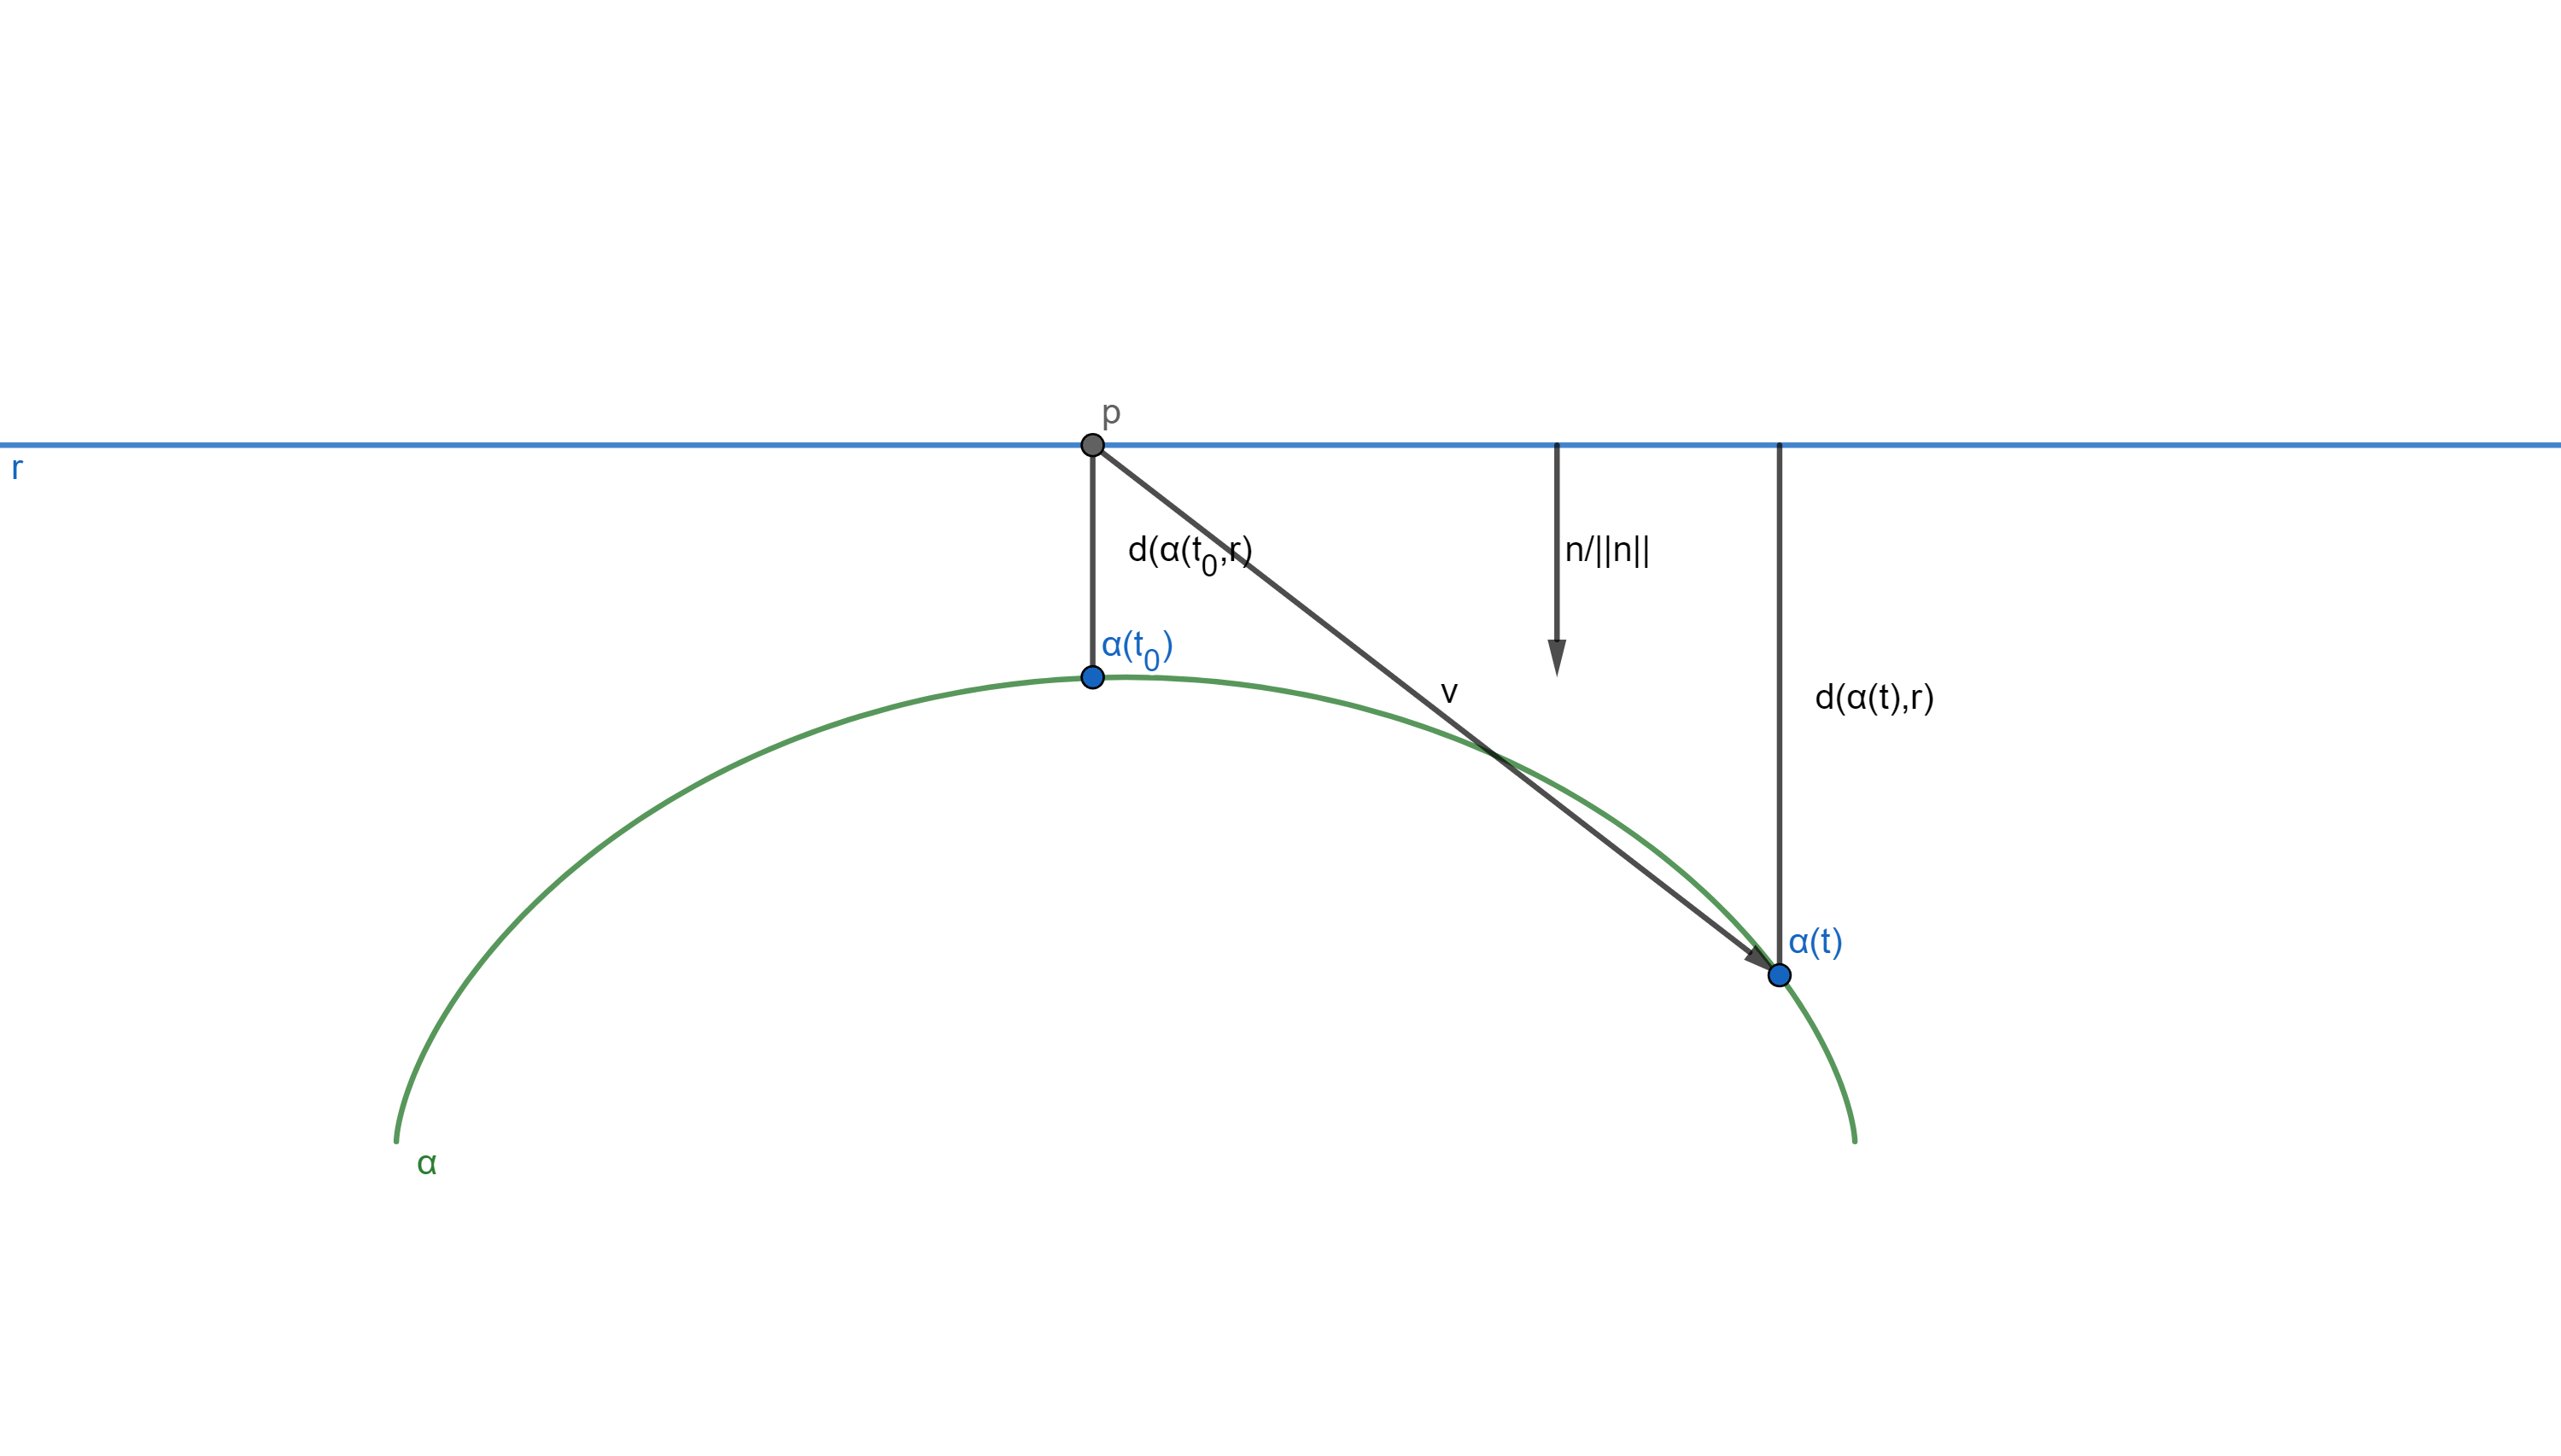
\includegraphics[]{figuras/geogebra-export.png}\\
    %\url{https://www.geogebra.org/calculator/qazc9dkm}
\end{center}
\end{document}
